\documentclass{beamer}
\usepackage{tikz}
\usepackage[UTF8]{ctex}
\begin{document}
\usetikzlibrary{calc}

\begin{tikzpicture}
    \fill(0,0) circle(1ex);
\end{tikzpicture}
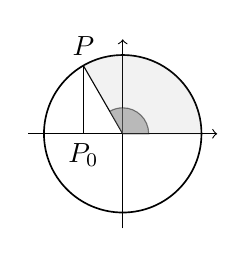
\begin{tikzpicture}
    \coordinate[label=above:$P$] (P) at (120:1);
    \coordinate[label=below:$P_0$] (P0) at (P|-0,0);
    \draw(0,0)--(P);
    \draw(P)--(P0);
    \draw[->](-1.2,0)--(1.2,0);
    \draw[->](0,-1.2)--(0,1.2);
    \draw[semithick](0,0) circle(1);
    %画实心扇面,扇面是由一条线段绕端点旋转得到。
    \filldraw[fill=gray,opacity=0.5] (0,0)--(0.33,0) arc(0:120:0.33);
    \filldraw[fill=gray,opacity=0.1] (0,0)--(1,0) arc(0:120:1);
\end{tikzpicture}
\begin{tikzpicture}
    \draw[thick](0,0) circle(2);
    \draw(-2,0)--(2,0);
    \coordinate[label=below:$S$] (S) at (0,0); %定义一个点
    \coordinate[label=225:$O$] (O) at (2,0);
    \draw[densely dashed](2,-3)--(2,3);
    \coordinate[label=above:$F$] (F) at (2,3);
    \coordinate[label=below:$F^\prime$] (Fprime) at (2,-3);
    \coordinate[label=135:$P^{\prime\prime}$] (Pprimeprime) at(20:2);
    \draw(S)--(Pprimeprime);
    \fill(Pprimeprime) circle(0.05);
    \coordinate[label=above:$P^{\prime}$] (Pprime) at(100:2);
    \draw[->](S)--(Pprime);
    \fill(Pprime) circle(0.05);
    \coordinate[label=above:$P$] (P) at(120:2);
    \draw[->](S)--(P);
    %画实心圆,实现点加粗的效果。
    \fill(P) circle(0.05);
    %计算中点
    \coordinate[label=45:$T$] (T) at($ (Pprime)!0.5!(Pprimeprime) $);
    \draw[dotted](S)--(T);
    %画两端带箭头的圆弧
    \draw[<->] (20:0.4) arc(20:60:0.4);
    \draw[<->] (60:0.4) arc(60:100:0.4);
    \coordinate[label=30:\tiny{$\delta$}](delta) at(40:0.4);
    \coordinate[label=90:\tiny{$\delta$}](delta) at(80:0.4);
    %以下六行代码为计算线段的外延点,并作延长线。
    \coordinate[label=0:$G^\prime$] (Gprime) at($ (Pprime)!1.4!(Pprimeprime) $);
    \coordinate[label=90:$G$] (G) at($ (Pprime)!-0.4!(Pprimeprime) $);
    \draw[](G)--(Gprime);
    \coordinate[label=0:$Q^\prime$] (Qprime) at($ (P)!1.2!(O) $);
    \coordinate[label=270:$Q$] (Q) at($ (P)!-0.2!(O) $);
    \draw[](Q)--(Qprime);
    \coordinate[label=180:$\textbf{S}$](S_vector) at(120:1.1);
    \draw[->](-2.9,0)--(-2.3,0);
    \coordinate[label=90:$\textbf{S}_0$](S0_vector) at (-2.6,0);
\end{tikzpicture}
\end{document}